%\mychapter{2}{previouswork}

\section{Previous work and theoretical background}
In this section, we review several previous works.
First, we provide some mathematical neuroscience models of representing action potentials such as spike trains, the neural response function and point-processes. Second, we review analyses based on multi-unit single-trial and single-trial multiple trial analyses highlighting the strength and weaknesses of each approach. Third, we review some existing state-of-the-art dimensionality
reduction techniques and their role in analyzing large scale neural recordings.
Finally, we review two spike train metrics that have been used to study neuronal
variability.

\subsection{Representation of spike trains}
Even if the size, shape and amplitude of action potentials is somewhat different,
action potentials are often viewed as identical events which occur at a single moment in time. A spike train is an increasing sequence of recorded times at which a neuron fires an action potential. Spike trains are considered as the main mode of information transmission in the nervous system.
%Formally, a spike train for  a single neuron labeled j is a sequence of spike times T$_{i}^{j} = \{t_{1}^{j}, ....., t_{n_{i}}^{j} \} = \{t_{i}^{j}\}$ where $0 \leq t_{1}^{j} < t_{2}^{j}< ... < t_{n_{i}}^{j} \leq T$  and  $n_{i} \geq 0$ is the number of spikes in the spike train.\\
Formally, a spike train is a sequence of spike times

$\displaystyle  \{t_{1}, ....., t_{n} \} = \{t_{i}\}_{i=1}^{n} \ \ 
 \text{with} \ \  0 \leq t_{1} < t_{2}< ... < t_{n} \leq T,$
 where n is the number of spikes in the sequence.
In this definition, the start and end times of the duration over which spikes are recorded is 0 and T respectively. There are various ways of representing spike trains. One way is through a raster plot, (see figure \ref{fig:Raster}).\\
 
 \begin{figure}[H]
  \centering
    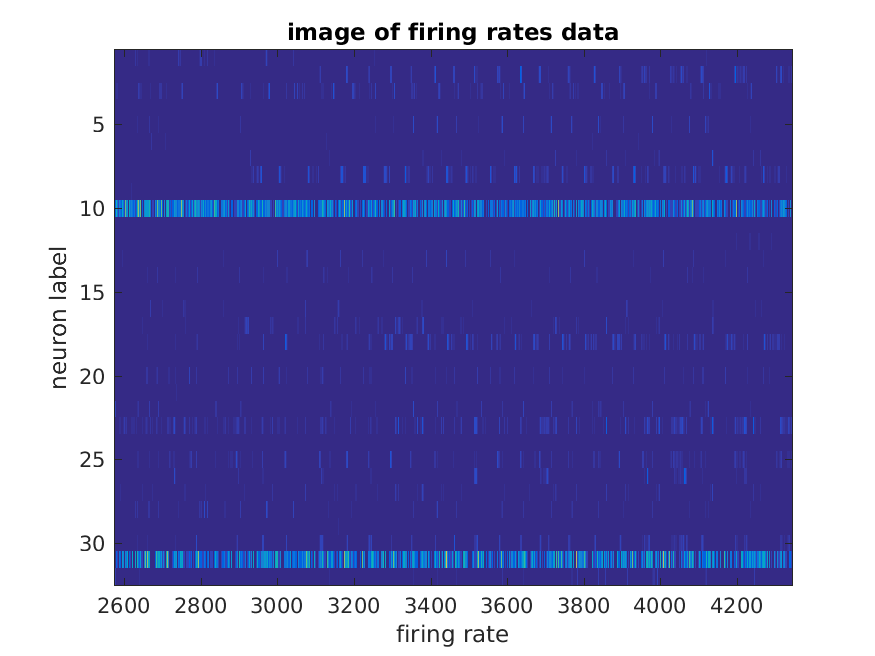
\includegraphics[scale=0.5]{/home/tesylvia/Oral_Sept_2017/images/RasterPlot.png}
     \caption{Raster plot for real-world data from a rat hippocampus}
     %label the figure so latex can reference it
      \label{fig:Raster}
\end{figure}

A spike train can also be represented as a sum of Dirac $\delta$ functions translated to the right by given spike times \cite{Dayan2001}.

%\begin{equation}\label{spiketrain}
% T_{i}^{j}(t) =: \sum_{i=1}^{n_{i}} \delta(t-t_{i}^{j})  
%\end{equation}
%Equation \eqref{spiketrain} represents the spike train $T_{i}^{j}$ of the $j^{th}$ neuron consisting of $n_{i}$ spikes occurring at times $t_{i}^{j}, i = 1 \ldots n_{i}$ where $t_{i}^{j}$ denotes the $i^{th}$ spike time of the $j^{th}$ neuron.  $T_{i}^{j}$ is referred to as the response function.\\

\begin{equation}\label{spiketrain}
 \rho(t) = \sum_{i=1}^{n} \delta(t-t_{i})  
\end{equation}
Equation \eqref{spiketrain} represents the spike train, of a single neuron, in a single trial, consisting of n spikes, occurring at times $t_{i}, i = 1 \ldots n$ where $t_{i}$ denotes the $i^{th}$ spike time of the cell.  
$\rho(t)$ is referred to as the neural response function.\\


The Dirac  function denoted $\delta(x)$ is defined by
\begin{Def}
\[
  \delta(x) =
  \begin{cases}
                                   0 & \text{if $x \neq 1$} \\
                                   \infty & \text{if $x=0$} 
  \end{cases}
\]
\end{Def}
As a "measure" on $\mathbb{R}$, we define
\begin{equation} \label{DiracDelta}
\displaystyle \int_{\mathbb{R}}  \delta(x)f(x) \quad dx = f(0) 
\end{equation}
where $f$ is any continuous function which vanishes outside a closed 
and bounded domain.\\

The  spike train \eqref{spiketrain} can also be represented as a continuous function of time, R(t), by filtering (convolving) with a Kernel K as shown below:

\begin{align*}
\displaystyle
R(t) = \rho(t)*K(t) &= \int_{\mathbb{R}} \rho(t-s)K(s)  ds \\
& = \int_{\mathbb{R}}    \sum_{i=1}^{n} \delta(t - s -t_{i}) K(s)  ds  \\
& =  \int_{\mathbb{R}}    \sum_{i=1}^{n} \delta( -(s - t + t_{i})) K(s)  ds\\
& =  \sum_{i=1}^{n}   \int_{\mathbb{R}} \delta(s - (t - t_{i})) K(s)  ds \quad (\text{ since $\delta(x)$ is even and we have a finite sum})\\
& = \sum_{i=1}^{n} K(t-t_{i}) 
\end{align*}

Thus
\begin{equation} \label{firerate}
R(t) = \sum_{i=1}^{n} K(t-t_{i})
\end{equation}




%\begin{align*}
%\displaystyle
%R^{j}(t) := T_{i}^{j}(t)*K(t) &= \int_{\mathbb{R}} T_{i}^{j}(t-s)K(s)  ds \\
%& = \int_{\mathbb{R}}    \sum_{i=1}^{n_{i}} \delta(t - s -t_{i}^{j}) K(s)  ds 
%\quad \eqref{spiketrain}  \\
%& =  \int_{\mathbb{R}}    \sum_{i=1}^{n_{i}} \delta( -(s - t + t_{i}^{j})) K(s)  ds\\
%& =  \sum_{i=1}^{n_{i}}   \int_{\mathbb{R}} \delta(s - (t - t_{i}^{j})) K(s)  ds \quad (\text{ since $\delta(x)$ is even and we have a finite sum})\\
%& = \sum_{i=1}^{n_{i}} K(t-t^{j}_{i}) \quad \eqref{DiracDelta}
%\end{align*}
%
%Thus
%\begin{equation} \label{firerate}
%R^{j}(t) = \sum_{i=1}^{n_{i}} K(t-t^{j}_{i})
%\end{equation}
%The function $R^{j}(t)$ is often referred to as the firing rate of the $j^{th}$ neuron. 
%Note that $R^{j}(t)$ is independent of the precise timing of a spike.
%Smoothing equation \eqref{spiketrain} with a kernel K enables us to represent events like spikes as continuous functions of time. R$^{j}$(t) is then viewed as an element of the infinite dimensional vector space of continuous functions.  Equation \eqref{firerate} 
%is also referred to a filtered spike train in spike metrics literature.
%The function $R^{j}(t)$ can also be viewed as an estimate of the unknown stimulus.
%(cite van Rossum's paper). 
%The common kernels used for estimating the firing rate include the Gaussian kernel,  decaying exponential kernel and Box car window.

% write an equation of these kernels and define what a kernel means
% copy and paste this from the kernel review you wrote on Xu's unpublished work.


\subsubsection{Derivation of the time varying firing rate}

Using equations \eqref{spiketrain} and \eqref{DiracDelta}, we obtain the total the number of spikes in the train by integrating the response function 
\begin{align*}
\int_{\mathbb{R}}  \rho(t)  dt &=   \int_{0}^{T}  \rho(t)  dt\\
      &= \displaystyle  \sum_{i=1}^{n}    \int_{0}^{T}  \delta(t-t_{i}) dt\\
              & = \displaystyle  \sum_{i=1}^{n} 1 = \text{n}
\end{align*}


Thus the spike-count rate, r,  on the interval [0, T]  given by

\[ \dfrac{\text{the number of spikes over the time interval of length T }}{T} \]

can also be expressed as the average of the neural response function
over a single trial of duration T

\begin{equation}\label{spike-count rate}
  \text{r} =  \frac{1}{T}  \int_{0}^{T}  \rho(t)  dt
\end{equation}

To reduce loss of temporal information due to averaging over a long period of time, the duration T of the experiment is often divided into small intervals [t, t+$\Delta$t] of length $\Delta$t so that the firing rate at time t,
denoted fr(t)  is  given by

\begin{equation}\label{single-trial emprical-spike count}
fr(t) = \dfrac{\text{number of spikes in the time interval} \quad [t, t+\Delta t]}
{\Delta t}
\end{equation}


\begin{Def}\label{trial-average neural response}
Let \text{M} be the total number of trials during an experiment
of multiple presentation of the same stimulus starting at time t=0 and to t=T. 
Let \[ \rho_{j}(t) = \displaystyle \sum_{i=1}^{n} \delta(t-t_{i})\] 
be the neural response function for the the j$^{th}$ trial for all j=1, $\dots$ M. The quantity 
\[ \langle \rho(t) \rangle  = 
\displaystyle  \frac{1}{M} \sum_{j=1}^{M} \rho_{j}(t)\] 

is called the trial-averaged neural response function

\end{Def}

The instantaneous time-varying firing rate, r(t), is the expectation of the 
trial-averaged neural response function over an infinite number of trials i.e.

\begin{equation} \label{expected FireRate}
r(t) = \displaystyle  \lim_{\Delta t \rightarrow 0}    \frac{1}{\Delta t}  \int_{t}^{t+\Delta t} 
 \langle \rho(t) \rangle \quad dt 
\end{equation}


In empirical experiments, the limit ${\Delta t \rightarrow 0}$ is usually
omitted since it's not possible to carry out an infinite number of experiments
in practice. Instead a sufficiently large number of trials is used
to estimate r(t), that is,

\[ 
r(t) \approx  \displaystyle  \frac{1}{\Delta t}  \int_{t}^{t+\Delta t} 
 \langle \rho(t) \rangle \quad dt 
\]

provided that there are enough spikes in the interval defining the r(t)
to yield a reliable estimate of the firing rate.

For a large $\Delta$t (long intervals), the average spike count denoted $\langle n  \rangle$ can then be  defined from the instantaneous firing rate as follows:

\begin{equation}\label{average spike count}
\langle n \rangle =  \displaystyle  \frac{1}{\Delta t}  
\int_{t}^{t+\Delta t}  r(t)  \quad dt 
\end{equation}

From equation \eqref{average spike count}, the average spike count is equivalent
to counting the number $n_{i}$  of spikes in the i$^{th}$ trial, for an infinitely large number of trials and taking the average of those spikes across the trials. This process of averaging spikes across trials is called trial-averaging.


However for short intervals around t such as $(t-\Delta t, t+\Delta t)$, the average spike count    $\langle n \rangle$ is approximately equal 
to r(t)$\Delta$t for small $\Delta$t.
In addition, $\Delta$t can be made arbitrarily small such that
the probability of getting more than one spike in the interval
 $(t-\Delta t, t+\Delta t)$ is zero. 
Hence in this interval, the average spike count is precisely the probability of getting one spike for sufficiently small $\Delta$t.


\subsubsection{Probabilistic interpretation of firing rate}
The probability of getting one spike in a short time interval  $(t-\Delta t, t+\Delta t)$ is equal to the value of the instantaneous firing rate, r(t) during that interval multiplied by the length of that interval, that is,

\[ 
\displaystyle  \text{p}(\{ \text{one spike during the interval interval} \quad  (t-\Delta t, t+\Delta t)  \}) = \text{r}(t)\Delta t. 
\]

\subsubsection{Short comings of using the firing rate}
First, the firing rate is an average of the neural response function over
multiple trials which gives only a partial description of the neuron's responses
unlike the spike train itself.
Second, the method of averaging across multiple trials is contrary to the way
the sensory system operates in general.
For instance a sequence of action potentials is sent from the optic nerves
to the brain which sends impulses to motor neurons so that muscles in eyes can close an animal's eye lids when a fly gets close to the eye's pupil.
The nervous system does not wait for the fly to get close to the pupil multiple
times before our eye lids shut to such a threat.
Thirdly, the firing rate does not take into account other patterns of spikes
that convey information such as the inter-spike intervals.
Thirdly, there are several underlying neural mechanisms such as cognition, memory
and olfaction which the experimentalist cannot control and hence cannot be extensively studied by presentation of controlled stimuli.
Finally, the firing rate r(t) determines the probability of getting one spike
in a short time interval $(t-\Delta t, t+\Delta t)$ but is generally not sufficient to determine the probability of getting an entire sequence of n spikes
in that short time interval.



\subsubsection{Point Processes}
A random variable is a number assigned to every outcome in an experiment.
For instance, the number of action potentials generated when an auditory neuron is stimulated
by a high pitched sound for 1.5ms or the number of heads obtained when a fair coin is tossed twice, are examples of random variables.  Each outcome in an experiment is generated according to some underlying probability distribution. A stochastic process is a collection  of random variables that vary with time such as the fluctuation of a voltage signal during an intracellular neuronal recording. A spike train is a sequence of recorded times at which a neuron fires an action potential. The rate at which a neuron fires a spike in a single trial (spike-count rate) is defined as the number of spikes obtained during that experiment divided by the duration of the experiment. The spike-count rate obtained from a single trial over a long duration, results into the smoothing over of rapid fluctuations of neuronal responses across that trial. To reduce this loss of temporal information, the duration of the experiment is divided into short time intervals [t, t+$\Delta$t] and action potentials are recorded repeatedly from neurons in response to the same stimulus.  The firing rate at time t, is then defined as the number of spikes recorded over the time interval of length $\Delta$t divided by the length of that interval. The instantaneous firing rate is then estimated by averaging spikes across a finite number of trials of the same experiment, a process also known as trial-averaging.\\

While analyses of neural activity in terms of the firing rate are useful in many contexts, certain changes in the pattern of spike times such as the variability of inter-spike intervals (ISIs) across spike trains may also covey information.
As much as the precise time at which a spike occurs is known to convey information, the stochastic behavior of gated-ion channels and the frequency of action potentials arriving at a synapse, may lead to varying neuronal responses.
For instance, spike times are highly variable even in controlled experiments like in vitro preparations where the same time-varying current is injected on multiple trials.
Thus the variability of ISIs observed in areas such as the cortex may be attributed to random processes that are unrelated to the stimulus or animal's behavior.\\


A stochastic process that generates irregular sequence of events such as spikes is called a point process. Let $\{t_{i} \}_{i=1}^{n}$ be a spike train of a single neuron consisting of
n spike times and $X_{i} = t_{i+1} - t_{i}$ be the inter-spike interval (ISI) recorded from
a time t=0 to T. Let $S_{j} = \sum_{i=1}^{j}X_{i}$ be the time of the j$^{th}$ spike.
The sequence $\{ S_{i} \}_{i \geq 1}$ forms a point process in the finite interval [0, T].




\subsubsection{The point process framework}
In the point-process framework, we view the neural response function as a point process. This implies that each spike train (a discrete event) consists of a sequence of spike times $\{t_{1}, \ldots, t_{n_{i}} \}$ which
are continuous random variables. Thus we know that each out come (spike train)
obtained during an intracellular recording is characterized by some underlying continuous probability density function. Denote this probability density function by p($\vect{t}$) where $\vect{t}$ denotes the vector of spike times $(t_{1}, \ldots t_{n})$. By the properties of a continuous random variable, the probability of obtaining a spike at time $t_{i}$ is equal to zero. Thus to obtain a non-zero probability, we seek the probability of obtaining a spike in a given time interval $(t_{i}, t_{i}+\Delta t)$ of length $\Delta$t.
Since we are assuming that each spike time $t_{i}$ is a stochastic random variable, it follows that  probability of getting one spike in a short time interval $(t_i, t_i+\Delta t)$ is equal to the product of  the probability density of $t_{i}$ also denoted by p(t$_{i}$) multiplied by the length 
of that interval ($\Delta$t), that is,

\[
\displaystyle \text{p}(\{\text{one spike during the interval} \quad (t_{i}, t_{i}+\Delta t) \}) = \text{p}(t_{i})\Delta t  
\]



Thus the expected spike count rate, the probabilistic (theoretical) counter part
of \eqref{single-trial emprical-spike count}, is given by

\begin{equation}\label{expected count rate}
\displaystyle 
\dfrac{\text{p}(\{\text{one spike during the interval} \quad (t_{i}, t_{i}+\Delta t)}{\Delta t} 
\end{equation}

Taking the limit as $\Delta t \rightarrow 0$, we obtain the expected instantaneous  firing rate
 
\begin{equation}\label{expected instant Firerate}
\displaystyle 
\text{FR}(t) =  \lim_{\Delta t \rightarrow t}  \dfrac{\text{p}(\{\text{one spike during the interval} \quad (t_{i}, t_{i}+\Delta t)}{\Delta t} 
\end{equation}


The beauty of the point process framework is that it provides a way of determining the probability of obtaining a sequence of n spikes i.e spike train.

Indeed, viewing the neural response function as a point process, the
probability of getting a sequence of n spikes in a short time interval
$(t_{i}, t_{i}+\Delta t)$ for all $i=1, \ldots n$ is given by the
product of the joint probability density of the random n-dimensional
vector of spike times p($t_{1}, \ldots, t_{n}$) multiplied by the quantity
$(\Delta t)^{n}$\\


\subsubsection{Non-homogenous poisson processes for spike simulation}
Still working on this...................


\subsection{Single-unit multiple trials}

Traditionally, experimentalists developed substantial scientific theories based on analyses from single-unit multiple-trial recordings. For instance, it is known that activity patterns from sensory neurons in the motor cortex of primates are tuned to the direction of the subject's arm movements \cite{Georgopoulos1982}, that neurons in the visual cortex of primates are tuned to the orientation of a stimulus \cite{Hubel1968}, that place cells in the CA1 region of the rat hippocampus are tuned to the animal's position in the environment \cite{OKeefe1971}, in addition to many others.
Classical  methods of analyzing single-unit recordings require averaging of responses across trials in order to estimate the firing rate from which information about the stimulus is decoded. Even though trial averaging may help reduce spiking variability, it does not reduce firing rate (response) variability.
Moreover, the process often results in the smoothing over of rapid fluctuations in the 
responses, which may lead to loss of temporal information in activity patterns, thus yielding incorrect interpretations of the underlying neural mechanisms.
In addition, there are neural mechanisms underlying certain observed phenomena 
that cannot be accounted for using single unit recordings.
For instance, consider that neither sensory neurons tuned to odor \cite{Hopfield1995},
nor certain internal mechanisms such as cognition and decision making (\cite{Redish2016,
Vos2015, Kaufman2014, Mazor2005}, can be controlled by researchers, as can other forms of external stimuli. Such observed phenomena, therefore, can only be analyzed by multiple-unit single-trial recordings. 




\subsection{Multiple-unit single trial}

On the other hand however, the use of multi-electrode \cite{Kipke2008} recording technologies has enabled  multiple-unit single-trial recording from various brain structures.\\
However, the challenge is that different neurons have highly heterogeneous patterns of activity (neuronal response variability) even on multiple presentation of the same stimulus. Trying to identify all possible activity patterns  corresponding to  a single neuron within the recorded neural population leads to an amplification in the number of variables to be considered while modeling collective neural responses. Consequently, biologically motivated assumptions have been made in order to model population activity. For instance, in the dynamical systems perspective, neurons belong to an underlying  tight recurrent connected network within the brain  which may favor correlated responses between neurons \cite{Shenoy2013}.
Among a population of neurons that encode features of a stimulus, the population activity is correlated with the features of the stimulus \cite{Georgopoulos1982, Hubel1968}.
Thus whether the researcher views the number of stimulus features as lower than the number of neurons in the population, or views neurons as belonging to an underlying network, it is nonetheless possible to study collective neural activity patterns using a low dimensional model which captures similar activity patterns among neuronal populations.\\

Lately, dimensionality reduction \cite{Cunningham2014a}, has been suggested as a tool for modeling population activity. Viewing the recorded N $>1$ neurons as measured variables in the data, dimensionality reduction provides a low dimensional model of the neural response space by finding a subset K $<<$ N of directions (dimensions) that explains most of the variability in the neuronal responses. Analyses on low dimensional neural population models have been be used to test scientific hypotheses about neural mechanisms that influence a subject's real-world experience. For instance, Mante et al. (2013) used Principle Component Analysis (PCA) and linear regression to show how sensory input is selected and integratedin the prefrontal cortex during decision-making   \cite{Vos2015}.  Kaufman et al. (2014) used Factor Analysis to show evidence of movement preparation before movement in the premotor cortex \cite{Kaufman2014}.  Mazor and Laurent (2005)  used PCA to demonstrate odor discrimination in the olfactory system \cite{Mazor2005}. In the context of exploratory data analysis and visualization, Yu et al. (2009) used Gaussian Process Factor Analysis (GPFA) to characterize single-trial population activity in  macaque premotor and motor cortices during reach planning and execution  \cite{Yu2009} .\\














%\begin{itemize}
%\item what are your long term objectives?
%\item Describe the model you've designed and the metric you're proposing to use
%\item How is this model and metric helping to address short comings of the previous model?
%\item What do you hope to accomplish with this new model?
%\item What new maths theories can be derived from this model?
%\item What are the applications to real world problems
%
%\end{itemize}






